\documentclass[../main.tex]{subfiles}

\begin{document}
\textbf{Note: grafer kan ses som formler fra \PRA, så bare brug F, G og H for
disse}
We will begin this section with define two classes of functions;
the \textit{Partial Recursive Functions} and  the \textit{Turing Computable
functions}. These two classes of functions gives rise to the same class of
functions The idea behind these two classes of functions is to define what
we intuitively mean with a computable function. The proofs in this section will
be rather informal. The goal of this section will be to state and prove
Kleene's recursion theorem, which will play a crucial role in our proof of 
Solovay's two  completeness theore

The topic I have chosen to call \textit{recursion theory} is today often known as
\textit{computability theory}. Robert Soares have stated some arguments for why this
name is better suited for the discipline than the name recursion theory in his
book \parencite{Soare2016}.

This sections will follow \parencite{Soare1987}, unless stated otherwise. 

\section{Partial Recursive Functions and Recursive Functions}
The class of partial recursive functions is an enlargement of the primitive recursive
functions. The class of primitive recursive functions capture a lot of the
function we intuitively sees as computable. It does not contain any function that
we would say was incomputable.

But the primitive recursive functions do not include all intuitively computable
functions. For example the following function, called the Ackermann function,  that is clearly computable is not
in the class of primitive recursive functions:
\begin{align*}
	Ack(0,n)&=n+1\\
	Ack(m+1,0)&=A(m,1)\\
	Ack(m+1,n+1)&=A(m,A(m+1,n))
\end{align*}

This function grows \textit{to fast} to be a primitive recursive function, i.e
we have for all primitive recursive functions $f(x)$ that for some $y$ that
$Ack(x,y)>f(x)$ for all $x\in \omega$. 
proof of this fact can be found in \textbf{Find ref}.

So we will need to expand our class of functions, if we want to
\textit{capture} all intuitively computable functions. 
We will expand them in the following way:
\begin{defi}
		The class of \textit{partial recursive} (from now on some times
		called (p.r) functions is the least class closed under schemata
		I through V from the definition of primitive recursive
		functions and the following VI schema . 
		\begin{enumerate}[label=\Roman*., start=6]
			\item If $\theta(\x,y)$ is a partial recursive function
				of $n+1$ variables and 
				\begin{align*}
					\psi(\x)=\mu
					y&[\theta(\x,y)\downarrow=0\\
						&\wedge \forall z\leq y
					[\theta(\x,z)\downarrow]
				\end{align*}
				Then $\psi$ is a partial recursive function of
				$n$ variables
		\end{enumerate}
		A partial recursive function that is total is called a total
		recursive function; abbreviated to recursive function.
\end{defi}

This is one way in which one can define what the computable functions are. In
the next section we will come with another definition of a type of functions,
and it will be shown that these leads to the same class of functions.

We will end this section with the following definition:
\begin{defi}
	A relation $R\subset\omega^n$ where $n\geq 1$, is recursive (primtive
	recursive) if its characteristic function $\chi_R$ is recursive
	(primitive recursive). The case where $n=1$ is the case where $R$ is a
	set $A\subset\omega$ so we also have the definition of a set being
	recursive.
\end{defi}

\section{Turing Computable Functions}

Another way to describe the intuitively computable functions is via a Turing
machine. 
\begin{defi}
	A \textit{Turing machine} $M$ consists of a two-way infinite tape that
	is dived into different cells and a finite set of internal states $Q=\{
	q_0,\ldots, g_n\}$, $n\geq 1$. Each cell  is either blank: B or has
	value 1.
	The following three things can happen in a single
	step:
	\begin{enumerate}
		\item Change form one state to another.
		\item Change the scanned symbol $s$ to another symbol
			$s'\in S=\{1,B\}$
		\item Move the reading head one cell to the right R or the left
			L.
	\end{enumerate}
	The operation of $M$ is controlled by a partial map:
	$$\delta:Q\times S\rightarrow Q\times S\times\{R,L\}$$
	Which may not be defined for all arguments.
\end{defi}
The situation can be seen in the following figure:
\begin{center}
	\begin{figure}[h]
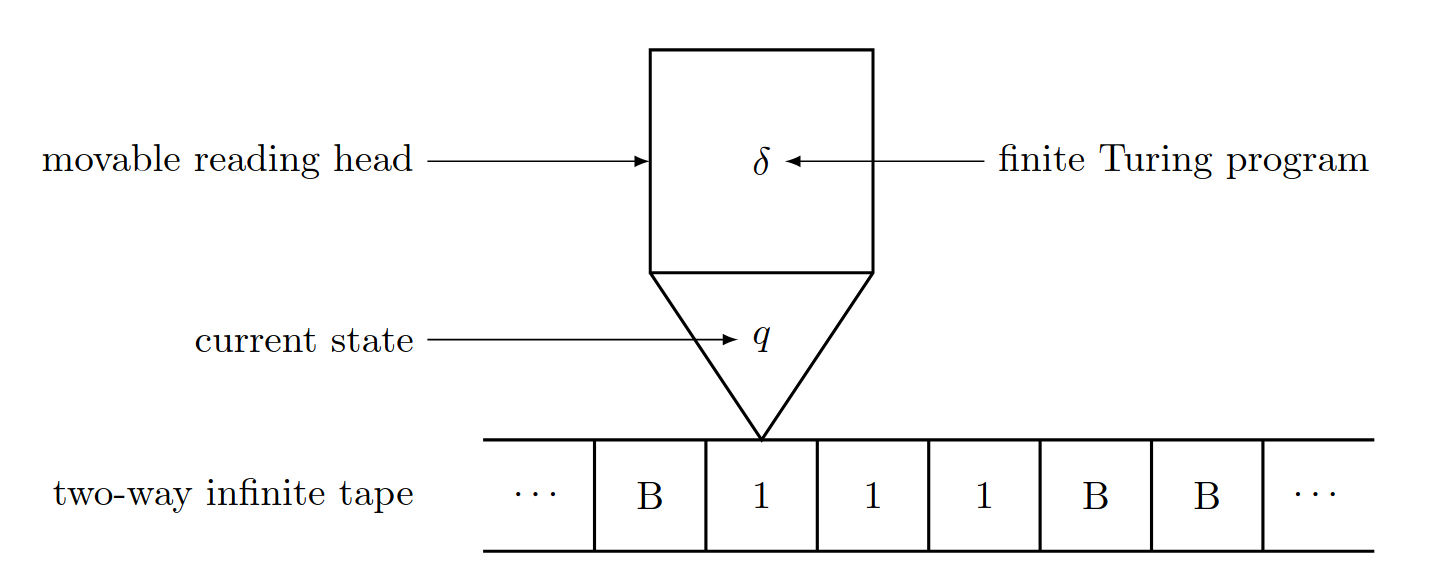
\includegraphics[width=\textwidth]{Turnig.png}
\caption{A Turing Machine}
\end{figure}
\end{center}

The way to understand this definition is the following: if
$(q,s,q',s',X)\in\delta$ it means that the machine $M$ is in stage $q$ where it
scans symbol $s$ then changes to state $q'$ and replaces $s$ by $s'$. Lastly it
moves to the right if $X=R$ and the left if $X=L$. The map $\delta$ is called a
Turing program if it can be views as a finite set of quintuples. If the input
integer is $x$ then it will be represented by a string of $x+1$ consecutive
$1's$, where all other cells are blank.

Further the machine $M$ start in the state $q_1$ scanning the left-most cell
that contains a $1$. The machine stops if it reaches the halting state $q_0$,
and it will then output the number $y$ which is the total number of $1$'s on
the tape in the this state. If $M$ with input $x$ halts and outputs $y$ we
say that $M$ computes the partial function $\psi(x)=y$

The conditi [Indfør noget mere tekst her]on a is determined by:
\begin{enumerate}
	\item The current state $q_i$
	\item The symbol $s_0$ that is being scanned.
	\item The symbols on the tape to the right of $s_0$ up to the last $1$.
		Denote this sequence by $s_1,s_2,\ldots s_n$
	\item The symbols on the tape to the left of $s_0$ op to the first $1$.
		Denote this sequence by $s_{-1},s_{-2},\ldots s_{-m}$
\end{enumerate}
This is called the configuration of the machine and we can write it as follows:
$$s_{-m}\cdots s_{-1}q_0s_0s_1\cdots c_n$$

\begin{defi}
	A Turing computation according to to the Turing program $P$ with input
	$x$ is a sequence of configurations $c_0,c_1,\ldots, c_n$ such that
	$c_0$ represent the machine in the halting state $q_0$, and the
	transition $c_i\rightarrow c_{i+1}$ for all $i<n$ is giving by the
	Turing program $P$.
\end{defi}

\begin{prop}
	Each Turing program $P_e$ can be assigned a Gödel number $e$.
\end{prop}
\begin{proof}
	We will use the fact that each $x\in\omega$ has a unique
	prime decomposition:
	$$x=p_0^{x_0}\cdots p_n^{x_n}\cdots$$
	We can assign a number to each quintuple $(q_i,_j,q_k,s_l,r_m)$ in a
	Turing program $P$ in the following way[Omformuler denne sætning]:
	$$p_0^{1+i}p_1^{1+j}p_2^{1+k}p_3^{1+l}p_4^{1+m}$$
	Where we have that $r_0=R$ and $r_1=L$. Since the prime decomposition
	is unique, each different state of the program has a unique code. Each Turing
	is a sequence of different states and we can thus for an arbitrary
	Turing program $P_e$ we let $e_0,\ldots e_n$ denote the Gödel number of
	each different state and set:
	$$e=p_0^{e_0}\cdots p_n^{e_n}$$
	Thus each Turing program $P_e$ has a unique Gödel number $e$.
\end{proof}
Since each Turing program has a unique code we can list them and be able to
find any program $P_e$ by its code $e$. This gives the following definition:
\begin{defi}
	The $P_e$ be the Turing program with Gödel number $e$ in the list and
	let $a_e^{(n)}$ be the function of $n$ variables computed by $P_e$.
	Further let $a_e$ abbreviate $a_e^{(1)}$.
\end{defi}
\section{The \textit{s-m-n}-Theorem}

It can be proven that the two classes of functions; partial recursive and Turing
computable functions gives rise to the same class of partial functions. This
can be seen as evidence for \textit{Church's Thesis} which states that this
class of functions coincide with the function that we see as intuitively
computable. In the rest of this project we will assume that the Church's Thesis
is true.

We will being by proving the padding lemma, which states that each partial
function $\varphi_x$ has an infitine amount of indices.
\begin{lem}[The Padding Lemma]
	Each partial recursive function $\varphi_i$ has $\aleph_0$ indicies,
	and for each $x$ we can \textit{effectively} find an infinite set $A_x$
	of indices for the same partial function.
\end{lem}
\begin{proof}
	For any program $P_x$ that have internal states: $\{q_0,\ldots, q_n\}$
	we can add extra instructions $q_{n+1}B\ R ,q_{n+2}B\ R,\ldots$ such
	that we get a new program for the same computation.
\end{proof}

The following theorem will show that each Turing computable function is in fact
partial recursive. The converse also holds and the proof of this fact can be
found in \parencite{Kleene1952}

\begin{thm}[The Normal Form Theorem]
	\label{thm:Normalform}
	There exist a predicate $T(e,x,y)$ and a function $U(y)$ that are
	primitive recursive such that:
	$$\varphi_e(x)=U(\mu yT(e,x,y))$$
\end{thm}
\begin{proof}
	We showing that the predicate $T(e,x,y)$ exists and is primitive
	recursive. This predicate informally
	states that $y$ is the code of Turing program $P_e$ with input $x$. For
	each possible configuration $c$, we can assign a code:
	$$\#(c)=2^{1+i}3^{1+\#(s_0)}5^r7^l$$
	Where $\#(s)=0$ if $s=B$ and is equal to $1$ otherwise, $r=\prod_{j\geq
	1}p_j^{\#(s_j)}$ and $l=\prod_{j\leq -1}p_j^{\#(s_j)}$
	 We can now define the code of a Turing computation
	$c_0,c_1,\ldots c_n$ according to $P_e$ to be:
	$$y=2^e\prod_{i\leq n}p_{i+1}^{\#(s_i)}$$
	We can now define $T(e,x,y)$ to be [Læs i Kleene]
	Having defined the predicate $T$ we can check if it holds. By
	proposition 2.1 we can "recover" the program $P_e$ form $e$. Then we
	can recover the computation $c_0,c_1,\ldots c_n$ form $y$ if $y$ codes
	such a thing. We can now check if $c_0,c_1,\ldots,c_n$ is a computation
	according to $P_e$ with $x$ as the input in the first configuration
	$c_0$. If this is true, then $U(y)$ just outputs the number of $1$'s in
	the final configuration $c_n$. [Læs mere i Klenne]
\end{proof}
This theorem also gives us that each partial recursive function can be created
by two primitive recursive functions, with a single application of the
$\mu$-operator.

\begin{thm}[Enumeration Theorem]
	\label{thm:Emu}
	There is a partial recursive function of $2$ variables
	$\varphi_z^{(2)}(e,x)$ such that $\varphi_z^{(2)}(e,x)=\varphi_e(x)$.
\end{thm}
\begin{proof}
	By Theorem \ref{thm:Normalform} we will define
	$\varphi_z^{(2)}(e,x)=U(\mu y T(e,x,y))=\varphi_e(x)$
\end{proof}
We will need the following notation in the next proof:
\begin{defi}
	Set $\la x,y\ra$ to be the image of $(x,y)$ under the injective
	recursive  pairing function:
	$$\frac{1}{2}(x^2+2xy+y^2+3x+y)$$
	This function is from $\omega\times\omega$ onto $\omega$.
\end{defi}
\begin{thm}[s-m-n theorem]
	For every $m,n\geq 1$ there exists an injective recursive function
	$s_n^m$ of $m+1$ variable such that for all $x,y_1,\ldots,y_m$
	$$\varphi^{(n)}_{s^m_n(x,y_1,\ldots,y_m)}=\lambda z_1,\ldots
	z_n[\varphi^{(m+n)}_x(y_1,\ldots,y_m,z_1,\ldots,z_n)]$$
\end{thm}
\begin{proof}
	I will follow Soare and only proof the case where $m=n=1$. I.e the case
	where we have to proof:
	$$a_{s^1_1(x,y)}(z)=[a_x^{2}(y,z)]$$
	Let $x$ and $y$ på given. Then $s^1_1(x,y)$ can be described as
	follows:
	\begin{enumerate}
		\item Let $P_x$ the Turing program with code $x$.
		\item Change $P_x$ into another Turing program $P_{x'}$ such
			that: $P_{x'}$ writes $y+1$ "1" left of the input, such
			that there is a B between these 1 and the other input.
			Further i places the head to the left of the new input
			and proceeds to \textit{run} $P_x$.
		\item outputs $x'$
	\end{enumerate}
	it is clear that $P_{x'}$ on input $z$ compute the same as $p_e$ would
	on input $(x,y)$; i.e $\varphi_{x'}=\varphi_x^{(2)}(y,z)$. Further we
	have that $x'=s^1_s(x,y)$
	By Church's Thesis the function $s=s^1_1$ is recursive, since it can be
	computed effectively. If it is not injective it can be replaced by a
	injective recursive function $s'$ such that
	$\varphi_{s(x,y)}=\varphi_{s'(x,y)}$ by using the padding lemma and by
	defining $s'(x,y)$ in increasing order of $\la x,y\ra$.
\end{proof}

A full proof of this statement can be found in Kleene. The $s-m-n$ theorem
plays a crucial role in both the proof and the use of the recursion theorem.
\textbf{Skriv noget om intuiton}. Therefore we will use the $s-m-n$ theorem to
prove the following proposition:
\begin{prop}
	There is a recursive function $g$ of two variables such that for all
	$x,y$:
\[\varphi_{g(x,y)}=\varphi_x\varphi_y\]
\end{prop}
\begin{proof}
	By Church's Thesis it is clear that $\eta=\varphi_x\varphi_y$ is a
	partial recursive function since it is the product of two partial
	recursive functions.

	To end the proof we must show that we can find Gödel number for $\eta$
	in an uniform effective way from $x$ and $y$ as $x$ and $y$ vary. We
	will start of by defining:
	\[\theta(x,y,z)=\varphi_x(\varphi_y(z))=\varphi_{x_1}(x,\varphi_{x_1}(y,z))\]
	Where $\varphi_{x_1}$ is the function $\varphi_z^{(2)}$ from Theorem
	\ref{thm:Emu}. By the church thesis this function is partial recursive
	and has an index $e$. So by applying the $s-m-n$ Theorem we get:
	\[\varphi_x\varphi_y=\lambda
	z[\varphi_e(x,y,z)]=\varphi_{s_1^2(e,x,y)}\]
	And thus $s_1^2(e,x,y)$ is our $g$ (i.e $\lambda xy[s_1^2)e,x,y)]$.
\end{proof}
\section{Recursively Enumerable sets and the Graph of a function}
In this section we will introduce the two concepts \textit{recursive
enumerable} sets and the \textit{graph} of a function. We will further show
that there is connection between these two concepts.
\begin{defi}
	A set $A$ is \textit{recursively enumerable} (r.e.) if $A$ is the domain of some
	primitive recursive function. Further we define the following two sets:
	\begin{enumerate}
		\item We let the $e$th r.e set be denoted by:
			$$E_e=\text{dom}\ (\varphi_e)= \{x:f(x)\downarrow\}=\{x:\exists
			y T(e,x,y)\}$$
		\item \[E_{e,s}=\text{dom} (\varphi_{e,s})\]
	\end{enumerate}
\end{defi}
A set can be recursively enumerable without being recursive, which the
following two propositions shows:
\begin{prop}
	Let $K=\{x:\varphi_x(x)\ \text{converges}\}=\{x:x\in E_x\}$, then $K$
	is r.e.
\end{prop}
\begin{proof}
	We have that $K$ is the domain of the following primitive recursive
	function:
	\[\psi(x)=\begin{cases}
		x &\text{if}\ \varphi_x(x)\ \text{converges}\\
		\text{undefined} &\text{otherwise.}
	\end{cases}\]
	This function is primitive recursive by Church Thesis, since $\psi(x)$
	can be computed by program $P_x$ on input $x$, which outputs $x$ only
	if $\varphi_x(x)$ converges.
\end{proof}
\begin{prop}
	$K$ is not recursive
\end{prop}
\begin{proof}
	If $K$ where recursive we would that it had a recursive characteristic
	function $K_\chi$, and thus the following would be recursive:
	\[f(x)=\begin{cases}
		\varphi_x(x)+1 & \text{if } x\in K\\
		0 & \text{if } x\not \in K
	\end{cases}\]
	But we this $f$ can not be recursive since for all $x$ we have $f\not
	=\varphi_x$.
\end{proof}
\textbf{Forklar kort meningen med dette}.

Next goal is to show that the definition of a r.e sets is equivalent to the
definition that there is an algorithm that enumerates the members of it. We
will further also show that the definition of a r.e set is equivalent to the
set being $\Sigma_1$, which is a concepts that will play a bigger role later on
in this project.
\begin{defi}
	A set $A$ is the \textit{projection} of some relation $R\subseteq
	\omega\times\omega$ if $A=\{x:\exists y: R(x,y)\}$. We further say that
	a set $A$ is in $\Sigma_1$ form, if $A$ is the projection of some
	recursive relation $R\subseteq\omega\times\omega$.
\end{defi}
We can now show the following theorem:
\begin{thm}
	A set $A$ is r.e iff $A$ is $\Sigma_1$.
\end{thm}
\begin{proof}
	($\Rightarrow$) Since $A$ is r.e we have that $A=W_e=\text{dom} f_e$
	for some $e$. This means that:
	$$x\in W_e\Leftrightarrow\exists s(x\in W_{e,s})\Leftrightarrow \exists
	s(T(e,x,s))$$
	Since the relation $T$ is primitive recursive and we have that the set $A$
	is the projection a recursive relation.

	($\Leftarrow$) Let $A=\{x:\exists y(Rx,y)\}$ where $R$ is recursive. We
	then have that $A=\text{dom} f$ where $f(x)=\mu y(R(x,y))$ and thus $A$
	is r.e
\end{proof}
\textbf{Skriv noget metatekst}
\begin{thm}
	\label{thm:RecSigma}
	If there is a recursive relation $R\subseteq\omega^{n+1}$ and if we
	have the following set:
	$$A=\{x|\exists y_1\ldots\exists  y_n R(x,\y)\}$$
	Then the set $A$ is $\Sigma_1$
\end{thm}
\begin{proof}
	We will start of by defining the relation $S\subseteq\omega^2$ as
	follows:
	$$S(x,z)\Leftrightarrow R(x,(z)_1,\ldots,(z)_n)$$
	Where we have the following prime decomposition of $z$:
	$$z=p_1^{(z)_1}\cdots p_k^{(z)_k}$$
	Then the following equivalences holds:
	\begin{align*}
		\exists zS(x,z)&\Leftrightarrow \exists z R(x,(z)_1,\ldots
		(z)_n)\\
			       &\Leftrightarrow \exists y_1\cdots \exists y_n
			       R(x,\y)
	\end{align*}
	And thus the set $A$ is clearly $\Sigma_1$.
\end{proof}
From this theorem we can easily get the following corollary:
\begin{cor}
	The projection of an r.e relation is r.e
\end{cor}

The next definition will also play a role in our proof of Solovay's
completeness theorems.

\begin{defi}
	The graph of a (partial) function $\varphi$ is the relation:
	\[(x,y)\in\ \text{graph} \varphi\Leftrightarrow f(x)=y\]
\end{defi}
The relation of a graph can also be seen as a function in the language of
$\PRA$; so we will often denote the graph of a function $\varphi(x)=y$ with the
following notation: $Fxy$, and say that $(x,y)\in\ \text{graph}(\varphi$ if and
only if $Fxy$ is true.

\begin{thm}
	If $R\subseteq\omega^2$ is an r.e relation, then there is a p.r
	function $\text{sel}$ called the selector function for $R$ such that:
	$$\text{sel}(x)\ \text{is defined}\ \Leftrightarrow\ \exists y(R(x,y))$$
	and if this is the case we have that $(x,f(x))\in R$
\end{thm}
\begin{proof}
	Since $R$ is r.e it is $\Sigma_1$. This means that there is a recursive
	relation $S$ such that $R(x,y)$ holds iff $\exists z (S(x,y,z))$. Thus
	we can define the following primitive recursive function:
	$$g(x)=\mu u(S(x,(u)_1,(u)_2))$$
	And now we put $f(x)=(g(x))_1$
\end{proof}
It will be the following theorem we will use in our proof later on.
\begin{thm}
	A partial function $\varphi$ is partial recursive iff its graph is recursive
	enumerable.
\end{thm}
\begin{proof}
	($\Rightarrow$) The graph of $\varphi_e$ is r.e by theorem \ref{thm:RecSigma} and the
	definition of a graph.

	($\Leftarrow$) Since the graph of $\varphi$ is assumed to be r.e we can
	conclude that $\varphi$ is its own primitive recursive selector function. This
	is that $R=\text{graph} \varphi$ can only have $\varphi$ as its selector function.
	[Whyyy?]
\end{proof}

\section{The Recursion Theorem}
In this section we will state and prove the recursion theorem. It will be
crucial in the next [chapter?], since we will need it to define a function.
\begin{thm}[The Recursion Theorem]
	For every recursive function $f$ there exists a fixed point $n$ such
	that $\varphi_n=\varphi_{f(x)}$
\end{thm}
\begin{proof}
	We will start of be defining the following \textit{diagonal} function
	$d(u)$ as:
	\begin{align}
		\label{eq:du}
		\varphi_{d(u)}(z)=\begin{cases}
		\varphi_{\varphi_u(u)}(z)& \text{if}\ \varphi_u(u)\
		\text{converges}\\
		\text{undefined} & \text{else}
	\end{cases}
	\end{align}
	By the $s-m-n$ theorem we have that the function $d$ is injective and
	total. Further it is clearly seen that $d$ is independent of $f$.

	Given an arbitrary $f$ we will choose an index $v$ such that:
	\begin{align}
		\label{eq:fd}
		\varphi_v=f\circ d
	\end{align}
	Now set $n=d(v)$. We will show that this is a fixed point for the
	function $f$. Since $f$ is total we also have that $f\circ d$ is total.
	This means that $\varphi_v(v)$ converges and that
	$\varphi_{d(v)}=\varphi_{\varphi_v(v)}$. Thus we have:
	$$\varphi_n=\varphi_{d(v)}=\varphi_{\varphi_v(v)}=\varphi_{f\circ
	d(v)}=\varphi_{f(n)}$$
	The second equality sign follows from \ref{eq:du} and the third follows
	from \ref{eq:fd}.
\end{proof}
Following [Owens, find ref], the argument in the proof can be seen as a
digitalization argument that fails. Commonly when we apply a digitalization
argument, we have a class of sequences, with terms from an set $A$, that we arranges as the rows in a square
matrix. We then have a map $h:A\rightarrow A$ that induces a operation $h^*$ on
the set of sequences such that if $\la s(i),i\in I\ra$ is a sequences in our
matrix then 
$$h^*(\la s(i),i\in I\ra)=\la h(s(i)),i\in I\ra$$
After having defined this map we will use it on the sequences that consists of
the elements of the  diagonal of the matrix and
show that the resulting sequences is not one of the original sequences. 

The digitalization argument "fails" in our case, since the sequences of the
diagonal is already already one of the rows and thus the image $h^*$ of this
sequences will also be one of the rows; i.e the $h$ has a fixed point.

The start of the proof can be seen as the following lemma:
\begin{lem}
	There is a diaognal function $d(u)$ such that:
	\begin{align}\varphi_{d(u)}(z)=\begin{cases}
		\varphi_{\varphi_u(u)}(z)& \text{if}\ \varphi_u(u)\
		\text{converges}\\
		\text{undefined} & \text{else}
	\end{cases}
	\end{align}
\end{lem}

Most of the times where one uses the Recursion Theorem, one actually uses this
lemma to construct the given function.

\subsection{Application of the Recursion Theorem}
The recursion theorem is a "powerful" tool. It enables us to define a partial
recursive function, which uses its own index as part of its definition. This
The recursion theorem overrides this "self-reference" because we are using the
$s-m-n$ theorem to define a function $f(x)$ and
$\varphi_{f(x)}(z)=(\ldots,x\ldots)$ and then taking a fixed point:
$\varphi_n=\varphi_{f(n)}$.  When we are making constructions like this the
only thing we cannot do is use specific properties of the function $\varphi_n$.
We will use the theorem in this way in our proof of Solovay's Completeness
Theorems to define a function with help of the functions own Gödel number; and
the recursion theorem makes this a viable tactic.

The
following examples will show a few uses of this theorem.
\begin{exmp}
	We will show that there is a $n$ such that:
	$$W_n=\{n\}$$
	We start of by using the $s-m-n$ theorem to define $W_{f(x)}=\{x\}$
	then by the recursion theorem we can choose $n$ such that we have:
	$$W_n=W_{f(n)}=\{n\}$$
\end{exmp}

The next example will be a application of the Recursion Theorem that is in the
same vein as the one we will use when we have to prove Solovay's completeness
theorems.
\begin{exmp}
	Let $\psi:\omega^2\rightarrow\omega$ and
	$\theta:\omega^3\rightarrow\omega$ be recursive functions and define
	the function $\varphi:\omega^2\rightarrow\omega$ by:
	\begin{align*}
		\varphi(0,y)&=\psi(y)\\
		\varphi(x+1,y)&=\theta(\varphi(x,y),x,y)
	\end{align*}
	We will now show that $\varphi$ is recursive by using the recursion
	theorem.

	Let $\phi_0 v_0v_1$ be an arbitrary graph and let $\phi_1v_0v_1$ be the
	graph of $\psi$ and $\chi v_0v_1v_2$ be the graph of $\theta$. We will
	now look at the following formula:
	\[\Phi(\phi_0):\ (v_0=\0\wedge \phi_1v_0v_1)\vee (v_0>\0\wedge \exists
	v(\phi_0(v_+-1,v)\wedge \chi vv_0v_1))\]
	We can see $\Godelnum{\Phi(\phi_0)}$ as a primitive recursive function
	of $\Godelnum{\phi_0}$. I.e we have:
	\[\Godelnum{\Phi(\phi_0)}=\eta(\Godelnum{\phi_0})\]
	We can now use the Recursion Theorem to chose a $n$ such that we have:
	$\varphi^{(2)}_{\eta(n)}=\varphi^{(2)}_n$ and for
	$varphi=\varphi^{(2)}_n$ we have:
	\[\varphi(x,y)=z\leftrightarrow(x=0\wedge\psi(y)=z=\vee(x>0\wedge
	\theta(\varphi(x-1,y),x,y)=z)\]
	I.e $\varphi$ does exactly what we want it to do. WE just need to
	define $\varphi$ and this can be done by a $\Sigma_1$ induction.
\end{exmp}

This ends our discussion about recursion theory. In the next chapter we will
generalize the notion of $\Sigma_1$ sets and in chapter \ref{chap:Complete} we
will use the recursion theorem to define a important function.

\end{document}
